\par\addvspace{12pt}\Needspace{9\baselineskip}

\section{复数与复平面}

\label{sol:sec:vector:5}

% ITEM: vector-complex-arithmetic
\solutionitem{vector-complex-arithmetic}{例3.13}
（1）计算\(\frac{3 + 4 i}{1 - 2 i}\)，并求它的模。


（2）解方程\(\left( z - 1 \right)^{2} + 4 = 0\)，在复平面上标出两个根。


（3）什么时候\(\left| z_{1} + z_{2} \right| = \left| z_{1} \right| + \left| z_{2} \right|\)？用图形说明。
\solutionanswer
（1）分子、分母同乘分母的共轭复数，得
\[
\frac{3+4i}{1-2i}
=\frac{(3+4i)(1+2i)}{5}=-1+2i.
\]
它的模为\(\sqrt{(-1)^2+2^2}=\sqrt5\)。

（2）由\((z-1)^2=-4\)，得到两个根\(z=1\pm2i\)，在复平面上对应点\((1,2)\)和\((1,-2)\)。
\begin{center}
\begin{tikzpicture}[scale=.68,>=stealth,font=\small]
\draw[->] (-1.1,0)--(3,0) node[right]{\(\operatorname{Re}z\)};
\draw[->] (0,-2.8)--(0,2.8) node[above]{\(\operatorname{Im}z\)};
\node[below left] at (0,0){\(O\)};
\draw[dashed,gray] (0,2)--(1,2)--(1,-2)--(0,-2);
\fill (1,2) circle(2pt) node[right]{\(1+2i\)};
\fill (1,-2) circle(2pt) node[right]{\(1-2i\)};
\node[below right] at (1,0){\(1\)};
\end{tikzpicture}
\end{center}
（3）若一个复数为零，等号成立。两者均非零时，将对应向量移到同一起点，记夹角为\(\theta\)，则
\[
|z_1+z_2|^2=|z_1|^2+|z_2|^2+2|z_1|\,|z_2|\cos\theta.
\]
所以等号成立当且仅当\(\cos\theta=1\)，即两个向量同向。图中两段沿同一方向首尾相接，总长度恰好等于两段长度之和：
\begin{center}
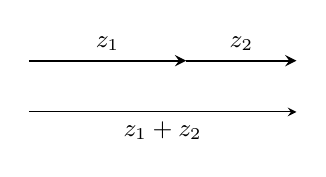
\begin{tikzpicture}[>=stealth,font=\small]
\draw[->,thick] (0,0)--(2,0) node[midway,above]{\(z_1\)};
\draw[->,thick] (2,0)--(3.4,0) node[midway,above]{\(z_2\)};
\draw[->] (0,-.65)--(3.4,-.65) node[midway,below]{\(z_1+z_2\)};
\end{tikzpicture}
\end{center}


% ITEM: vector-imaginary-unit-rotation
\solutionitem{vector-imaginary-unit-rotation}{思考：虚数单位与旋转}
分别用复数乘法与旋转变换解释\(i^{2} = - 1\)，并说明乘以\(- i\)对应怎样的变换。
\solutionanswer
由乘法定义，\((0+i)(0+i)=-1\)，故\(i^2=-1\)。

几何上，\(i(a+bi)=-b+ai\)，即\((a,b)\mapsto(-b,a)\)，对应逆时针旋转\(90^\circ\)。连续做两次得到\((a,b)\mapsto(-a,-b)\)，也就是乘以\(-1\)。乘以\(-i\)则为\((a,b)\mapsto(b,-a)\)，对应顺时针旋转\(90^\circ\)。


% ITEM: vector-elementary-complex-calculations
\solutionitem{vector-elementary-complex-calculations}{习题3.6（1）}
计算\((1+i)^8\)与\((1-i)/(1+i)\)。
\solutionanswer
由\((1+i)^2=2i\)，
\[
(1+i)^8=(2i)^4=16.
\]
又有
\[
\frac{1-i}{1+i}=\frac{(1-i)^2}{2}=-i.
\]


% ITEM: vector-sum-product-conjugate
\solutionitem{vector-sum-product-conjugate}{习题3.6（2）}
已知\(z+\overline z=4\)、\(z\overline z=13\)，求\(z\)。
\solutionanswer
设\(z=x+yi\)，其中\(x,y\)为实数。由\(2x=4\)得\(x=2\)，再由\(x^2+y^2=13\)得\(y^2=9\)。所以
\[
z=2+3i\quad\text{或}\quad z=2-3i.
\]


% ITEM: vector-perpendicular-bisector
\solutionitem{vector-perpendicular-bisector}{习题3.6（3）}
在复平面上画出满足\(|z-1|=|z+1|\)的点集。
\solutionanswer
\par\noindent
\begin{minipage}[c]{.68\linewidth}
\setlength{\parindent}{2em}
两边分别是动点到\(1,-1\)所对应两点的距离，故点集是连接这两点的线段的垂直平分线，也就是虚轴。

设\(z=x+yi\)，平方后相减得
\((x-1)^2+y^2=(x+1)^2+y^2\)，即\(x=0\)，与几何判断一致。
\end{minipage}\hfill
\begin{minipage}[c]{.29\linewidth}
\centering
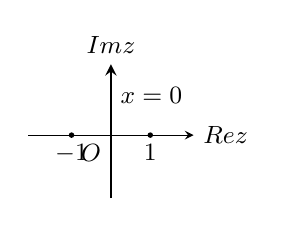
\begin{tikzpicture}[scale=.5,>=stealth,font=\small]
\draw[->] (-2.1,0)--(2.1,0) node[right]{\(\operatorname{Re}z\)};
\draw[->,thick] (0,-1.6)--(0,1.8) node[above]{\(\operatorname{Im}z\)};
\fill (-1,0) circle(2pt) node[below]{\(-1\)};
\fill (1,0) circle(2pt) node[below]{\(1\)};
\node[below left] at (0,0){\(O\)};
\node[right] at (0,1){\(x=0\)};
\end{tikzpicture}
\end{minipage}\par


% ITEM: vector-oblique-complex-basis
\solutionitem{vector-oblique-complex-basis}{例3.14 *}
在实基\(e_1=1,e_2=1+i\)下，求\(i\)的坐标与乘以\(i\)的变换矩阵，验证行列式不变。计算\(\langle e_1,e_2\rangle\)，说明坐标为\((1,0)\)、\((0,1)\)为何不足以判定正交。
\solutionanswer
由\(i=e_2-e_1\)，\(i\)在新基下的坐标为\((-1,1)\)。记乘以\(i\)的变换为\(L_i\)，则
\[
L_i(e_1)=i=-e_1+e_2,\qquad
L_i(e_2)=i(1+i)=-1+i=-2e_1+e_2.
\]
所以矩阵与行列式为
\[
[L_i]_{(e_1,e_2)}=
\begin{bmatrix}-1&-2\\1&1\end{bmatrix},
\qquad \det[L_i]_{(e_1,e_2)}=1.
\]
标准基\((1,i)\)下的矩阵为\(\begin{bmatrix}0&-1\\1&0\end{bmatrix}\)，行列式也为\(1\)。

另一方面，
\[
\langle e_1,e_2\rangle
=\operatorname{Re}(1\cdot\overline{1+i})=1\ne0.
\]
两个基向量在它们自身构成的基下总有坐标\((1,0),(0,1)\)，但坐标内积的简式只有在正交单位基下才成立，不能由这两个数组直接判定正交。


% ITEM: vector-parallelogram-norm
\solutionitem{vector-parallelogram-norm}{习题3.7（1） *}
由代数范数的表达式证明平行四边形恒等式
\begin{equation*}
 N(z+w)+N(z-w)=2N(z)+2N(w).
\end{equation*}
\solutionanswer
利用\(N(z)=z\overline z\)，展开得
\[
\begin{aligned}
N(z+w)&=N(z)+N(w)+z\overline w+\overline z w,\\
N(z-w)&=N(z)+N(w)-z\overline w-\overline z w.
\end{aligned}
\]
相加即得
\[
N(z+w)+N(z-w)=2N(z)+2N(w).
\]
对应到平面，便是平行四边形两条对角线长度的平方和，等于四条边长度的平方和。


% ITEM: vector-oblique-norm-inner-product
\solutionitem{vector-oblique-norm-inner-product}{习题3.7（2） *}
在基\(e_1=1,e_2=1+i\)下，设\(z=xe_1+ye_2\)、\(w=se_1+te_2\)。写出\(N(z)\)与\(\langle z,w\rangle\)关于\(x,y,s,t\)的表达式，比较它们与标准正交基下的公式。
\solutionanswer
先转回代数形式：
\[
z=(x+y)+yi,\qquad w=(s+t)+ti.
\]
因此
\[
\begin{aligned}
N(z)&=(x+y)^2+y^2=x^2+2xy+2y^2,\\
\langle z,w\rangle&=(x+y)(s+t)+yt
=xs+xt+ys+2yt.
\end{aligned}
\]
与标准正交基下的\(x^2+y^2,xs+yt\)相比，这里出现了交叉项，系数也改变了；变化来自所用基向量的长度与相互内积。


% ITEM: vector-multiplication-isometry
\solutionitem{vector-multiplication-isometry}{习题3.7（3） *}
设\(u\ne0\)。证明乘以\(u\)的变换保持正交关系，并求其逆变换的矩阵。它在什么条件下保持所有向量的长度？
\solutionanswer
由内积与乘法的关系，
\[
\langle uz,uw\rangle=|u|^2\langle z,w\rangle.
\]
由于\(|u|^2>0\)，变换前后的内积同时为零，故保持正交关系。

写\(u=a+bi\)，其逆变换为乘以
\[
\frac1u=\frac{a-bi}{a^2+b^2}.
\]
因此在基\((1,i)\)下，逆矩阵为
\[
\frac1{a^2+b^2}\begin{bmatrix}a&b\\-b&a\end{bmatrix}.
\]
由\(|uz|=|u|\,|z|\)，保持全部向量的长度当且仅当\(|u|=1\)。


% ITEM: vector-conjugation-map
\solutionitem{vector-conjugation-map}{习题3.7（4） *}
将共轭映射\(C(z)=\overline z\)看成实线性变换，求它在基\(1,i\)下的矩阵与行列式。它保持内积吗？能否找到固定复数\(u\)，使\(C(z)=uz\)对所有\(z\)成立？
\solutionanswer
共轭对实数的线性组合相容，故为实线性变换。由\(C(1)=1,C(i)=-i\)，矩阵及行列式为
\[
[C]_{(1,i)}=\begin{bmatrix}1&0\\0&-1\end{bmatrix},
\qquad\det[C]_{(1,i)}=-1.
\]
它保持内积，因为
\[
\langle\overline z,\overline w\rangle
=\operatorname{Re}(\overline z w)
=\operatorname{Re}(z\overline w)=\langle z,w\rangle.
\]
不存在所问的固定复数\(u\)。若存在，由\(z=1\)得\(u=1\)，但\(z=i\)时会要求\(-i=i\)，矛盾。


% ITEM: vector-complex-representations
\solutionitem{vector-complex-representations}{例3.15}
将\(- 1 + i\)，\(\sqrt{3} - i\)，\(- 2 i\)分别写成三角形式与指数形式，并指出它们的主辐角。
\solutionanswer
先求模，再由实部、虚部的符号确定辐角所在象限：
\[
\begin{aligned}
-1+i&=\sqrt2\left(\cos\frac{3\pi}4+i\sin\frac{3\pi}4\right)
=\sqrt2e^{3\pi i/4},\\
\sqrt3-i&=2\left(\cos\left(-\frac\pi6\right)+i\sin\left(-\frac\pi6\right)\right)
=2e^{-\pi i/6},\\
-2i&=2\left(\cos\left(-\frac\pi2\right)+i\sin\left(-\frac\pi2\right)\right)
=2e^{-\pi i/2}.
\end{aligned}
\]
主辐角依次为\(3\pi/4,-\pi/6,-\pi/2\)。


% ITEM: vector-exponential-periodicity
\solutionitem{vector-exponential-periodicity}{思考：复指数的周期性}
用模与辐角说明：\(e^{z_{1}} = e^{z_{2}}\)，当且仅当\(z_{1} - z_{2} = 2 k \pi i\)，其中\(k \in \mathbb{Z}\)。
\solutionanswer
写\(z_j=x_j+iy_j\)。由\(|e^{z_j}|=e^{x_j}\)，两指数值相等必有\(e^{x_1}=e^{x_2}\)，从而\(x_1=x_2\)。再比较方向，得到\(y_1-y_2=2k\pi\)，故
\[
z_1-z_2=2k\pi i,\qquad k\in\mathbb Z.
\]
反过来，若满足此条件，两个指数的模相同，辐角相差\(2k\pi\)，所以指数值相等。


% ITEM: vector-circle-under-multiplication
\solutionitem{vector-circle-under-multiplication}{思考：复乘法作用于圆}
乘以一个非零复数能将圆变成非圆的椭圆吗？
\solutionanswer
不能。设原圆为\(|z-z_0|=R\)，令\(w=cz\)，其中\(c\ne0\)。则
\[
|w-cz_0|=|c|\,|z-z_0|=|c|R.
\]
反过来也可除以\(c\)恢复原圆上的点。因此像仍是圆，圆心为\(cz_0\)，半径为\(|c|R\)。复数乘法在所有方向上使用同一个伸缩倍数。


% ITEM: vector-complex-versus-anisotropic
\solutionitem{vector-complex-versus-anisotropic}{思考：复乘法与方向伸缩 *}
将乘以非零复数的变换与前一节沿两个坐标方向作不同伸缩的变换比较。
\solutionanswer
乘以\(c=re^{i\theta}\ne0\)相当于统一伸缩\(r\)倍，再旋转\(\theta\)。其矩阵是
\[
rR_\theta=\begin{bmatrix}r\cos\theta&-r\sin\theta\\
r\sin\theta&r\cos\theta\end{bmatrix}.
\]
沿两坐标方向分别伸缩\(a,b>0\)的矩阵则为\(\operatorname{diag}(a,b)\)。若两矩阵相同，非对角元素要求\(\sin\theta=0\)，对角元素再要求\(a=b\)。此时可直接取正实数\(c=a\)。

因此方向伸缩在\(a\ne b\)时不能由一次复数乘法实现：它改变不同方向的长度比例，可将圆变成非圆椭圆；复数乘法则保持夹角，始终将圆变成圆。


% ITEM: vector-polynomial-factorization
\solutionitem{vector-polynomial-factorization}{例3.16 *}
已知实系数多项式\(P(z)=z^4-4z^3+8z^2-8z+4\)有根\(1+i\)。求它的全部根及各根的重数，并分别在实数与复数范围内分解因式。
\solutionanswer
系数为实数，所以\(1-i\)也是根。两个相应因式的乘积为
\[
(z-1-i)(z-1+i)=(z-1)^2+1=z^2-2z+2.
\]
由给定多项式除以这个二次式，商仍为同一二次式，故实数范围内的分解为
\[
P(z)=(z^2-2z+2)^2.
\]
复数范围内的分解为
\[
P(z)=(z-1-i)^2(z-1+i)^2.
\]
因此全部根为\(1+i,1-i\)，各为二重根。


% ITEM: vector-real-polynomial-parity
\solutionitem{vector-real-polynomial-parity}{习题3.8（1） *}
不使用连续性，由非实根成共轭对出现，证明每个实系数奇数次多项式至少有一个实根。偶数次多项式的实根总重数有什么特点？
\solutionanswer
设多项式次数为\(n\)，实根的总重数为\(r\)。非实根成共轭对出现，同一对的重数相等，所以非实根的总重数为某个偶数\(2m\)。

由代数基本定理及其分解推论，计重数的根共有\(n\)个，因此
\[
n=r+2m.
\]
\(n\)为奇数时，\(r\)为正奇数，故至少有一个实根；\(n\)为偶数时，\(r\)为偶数，也可以为零。


% ITEM: vector-polynomial-identity
\solutionitem{vector-polynomial-identity}{习题3.8（2） *}
设\(P,Q\)的次数都不超过\(n\)，且在\(n+1\)个不同的复数处取值相同。证明\(P=Q\)。
\solutionanswer
令\(R=P-Q\)。它在给定的\(n+1\)个互异复数处均为零。若\(R\)不是零多项式，其次数不超过\(n\)，不同的根却至少有\(n+1\)个，与多项式根数不超过次数矛盾。因此\(R=0\)，即\(P=Q\)。


% ITEM: vector-complex-powers-roots
\solutionitem{vector-complex-powers-roots}{例3.17}
（1）计算\(\left( 1 + i \right)^{10}\)。


（2）求方程\(z^{4} + 16 = 0\)的全部根，分别写出代数形式与指数形式，并在复平面上标出它们。
\solutionanswer
（1）由\(1+i=\sqrt2e^{\pi i/4}\)，
\[
(1+i)^{10}=2^5e^{5\pi i/2}=32i.
\]
（2）方程等价于\(z^4=-16=16e^{\pi i}\)。全部根为
\[
z_k=2e^{\,i(\pi/4+k\pi/2)},\qquad k=0,1,2,3.
\]
代数形式依次为
\[
\sqrt2+\sqrt2i,\quad-\sqrt2+\sqrt2i,\quad
-\sqrt2-\sqrt2i,\quad\sqrt2-\sqrt2i.
\]
\Needspace{10\baselineskip}
它们在半径为\(2\)的圆上构成正方形：
\begin{center}
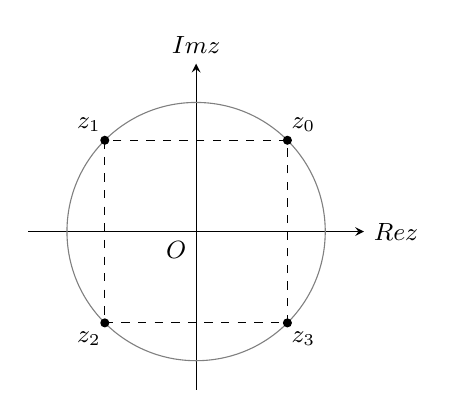
\begin{tikzpicture}[scale=.82,>=stealth,font=\small]
\draw[->] (-2.6,0)--(2.6,0) node[right]{\(\operatorname{Re}z\)};
\draw[->] (0,-2.45)--(0,2.6) node[above]{\(\operatorname{Im}z\)};
\draw[gray] (0,0) circle(2);
\draw[dashed] (45:2)--(135:2)--(225:2)--(315:2)--cycle;
\foreach \a/\k in {45/0,135/1,225/2,315/3}
  {\fill (\a:2) circle(2pt); \node at (\a:2.35){\(z_{\k}\)};}
\node[below left] at (0,0){\(O\)};
\end{tikzpicture}
\end{center}


% ITEM: vector-unit-root-sum
\solutionitem{vector-unit-root-sum}{思考：单位根的和}
设\(\omega = e^{2 \pi i / n}\)，\(n \ge 2\)。从运算与几何两方面说明\(1 + \omega + \cdots + \omega^{n - 1} = 0\)。
\solutionanswer
从运算看，\(\omega^n=1\)且\(\omega\ne1\)，所以
\[
(\omega-1)(1+\omega+\cdots+\omega^{n-1})=\omega^n-1=0.
\]
除以\(\omega-1\)，即得所求和为零。

从几何看，这些单位根在圆周上等距分布。把对应的所有位置向量相加，记所得向量为\(s\)。旋转\(2\pi/n\)使这些向量依次换位，因此它们的和仍是\(s\)。一个向量经过非整周旋转而保持不变，只能是零向量，故\(s=0\)。


% ITEM: vector-equilateral-complex
\solutionitem{vector-equilateral-complex}{例3.18}
点\(A , B , C\)分别对应\(a = 1 + i\)，\(b = 3 + i\)，\(c = 2 + \left( 1 + \sqrt{3} \right) i\)。用复数的模与辐角证明\(\triangle A B C\)是正三角形，并求其面积。
\solutionanswer
有
\[
b-a=2,\qquad c-a=1+\sqrt3i=2e^{\pi i/3}.
\]
所以两边\(AB,AC\)的长度都为\(2\)，从\(\vec{AB}\)到\(\vec{AC}\)的夹角为\(\pi/3\)，故三角形是正三角形。也可由\(|c-b|=|-1+\sqrt3i|=2\)直接核对第三条边。

面积为
\[
S=\frac12\cdot2\cdot2\sin\frac\pi3=\sqrt3.
\]


% ITEM: vector-complex-four-calculations
\solutionitem{vector-complex-four-calculations}{习题3.9（1）}
计算\(\left( 2 - i \right) \left( 1 + 3 i \right)\)，\(\frac{3 + 4 i}{2 - i}\)，\(i^{2026}\)，\(\left( 1 - i \right)^{12}\)。
\solutionanswer
依次计算：
\[
\begin{aligned}
(2-i)(1+3i)&=5+5i,\\
\frac{3+4i}{2-i}&=\frac{(3+4i)(2+i)}5=\frac{2+11i}5,\\
i^{2026}&=(i^4)^{506}i^2=-1,\\
(1-i)^{12}&=(\sqrt2e^{-\pi i/4})^{12}=64e^{-3\pi i}=-64.
\end{aligned}
\]


% ITEM: vector-conjugate-equation
\solutionitem{vector-conjugate-equation}{习题3.9（2）}
设\(z\)满足\(\left( 1 + i \right) z + \left( 2 - i \right) \overline{z} = 5 + i\)，求\(z\)。
\solutionanswer
设\(z=x+yi\)，则左边为
\[
(1+i)(x+yi)+(2-i)(x-yi)=(3x-2y)-yi.
\]
比较实部、虚部，得到\(3x-2y=5,-y=1\)，所以\(x=1,y=-1\)，即\(z=1-i\)。


% ITEM: vector-conversions
\solutionitem{vector-conversions}{习题3.9（3）}
将\(- 1 + \sqrt{3} i\)，\(1 - i\)，\(- 3 i\)分别写成三角形式与指数形式；将\(2 e^{3 \pi i / 4}\)，\(e^{- \pi i / 6}\)写成代数形式。
\solutionanswer
前三个数的三角形式与指数形式为
\[
\begin{aligned}
-1+\sqrt3i&=2\left(\cos\frac{2\pi}3+i\sin\frac{2\pi}3\right)=2e^{2\pi i/3},\\
1-i&=\sqrt2\left(\cos\left(-\frac\pi4\right)+i\sin\left(-\frac\pi4\right)\right)
=\sqrt2e^{-\pi i/4},\\
-3i&=3\left(\cos\left(-\frac\pi2\right)+i\sin\left(-\frac\pi2\right)\right)
=3e^{-\pi i/2}.
\end{aligned}
\]
后两个数的代数形式为
\[
2e^{3\pi i/4}=-\sqrt2+\sqrt2i,\qquad
e^{-\pi i/6}=\frac{\sqrt3}2-\frac12i.
\]


% ITEM: vector-real-imag-reverse-triangle
\solutionitem{vector-real-imag-reverse-triangle}{习题3.9（4）}
证明\(\operatorname{Re} z = \frac{z + \overline{z}}{2}\)，\(\operatorname{Im} z = \frac{z - \overline{z}}{2 i}\)，并证明\(\left| \left| z_{1} \right| - \left| z_{2} \right| \right| \le \left| z_{1} - z_{2} \right|\)。
\solutionanswer
写\(z=x+yi\)，便有\(z+\overline z=2x,z-\overline z=2yi\)，所以
\[
\operatorname{Re}z=\frac{z+\overline z}2,\qquad
\operatorname{Im}z=\frac{z-\overline z}{2i}.
\]
由三角不等式，
\[
|z_1|\le|z_1-z_2|+|z_2|,
\]
故\(|z_1|-|z_2|\le|z_1-z_2|\)。交换下标，又得相反差值的同一上界，两式合起来就是
\[
\bigl||z_1|-|z_2|\bigr|\le|z_1-z_2|.
\]


% ITEM: vector-product-quotient-arguments
\solutionitem{vector-product-quotient-arguments}{习题3.9（5）}
设\(z_{1} = 2 e^{5 \pi i / 6}\)，\(z_{2} = 3 e^{\pi i / 3}\)，求\(z_{1} z_{2}\)，\(z_{1} / z_{2}\)的模与主辐角。
\solutionanswer
乘法的模相乘、辐角相加，因此
\[
z_1z_2=6e^{7\pi i/6}=6e^{-5\pi i/6}.
\]
其模为\(6\)，主辐角为\(-5\pi/6\)。

除法的模相除、辐角相减，所以
\[
\frac{z_1}{z_2}=\frac23e^{\pi i/2}=\frac23i.
\]
其模为\(2/3\)，主辐角为\(\pi/2\)。


% ITEM: vector-complex-similarity
\solutionitem{vector-complex-similarity}{习题3.9（6）}
说明变换\(z \mapsto \left( \sqrt{3} + i \right) z\)的几何意义，求逆变换，并说明面积怎样变化。\optionalexercisepart{写出}它在基\(1 , i\)下的矩阵。
\solutionanswer
由于\(\sqrt3+i=2e^{\pi i/6}\)，这个变换把长度伸长为原来的\(2\)倍，并绕原点逆时针旋转\(\pi/6\)。若像为\(w\)，逆变换为
\[
z=\frac{w}{\sqrt3+i}=\frac{\sqrt3-i}{4}w.
\]
\Needspace{5\baselineskip}
面积变为原来的\(2^2=4\)倍。

\optionalexercisepart{矩阵为}
\[
\begin{bmatrix}\sqrt3&-1\\1&\sqrt3\end{bmatrix}.
\]
两列分别记录乘法作用于\(1,i\)后所得的坐标。


% ITEM: vector-centered-rotation-reflection
\solutionitem{vector-centered-rotation-reflection}{习题3.9（7）}
以\(1 + i\)为中心，将点\(3 + i\)逆时针旋转\(\pi / 2\)角，求像点的复数。再写出关于过原点、与实轴成\(\pi / 6\)角的直线作镜像的复数表达式。\optionalexercisepart{写出}镜像变换的矩阵。
\solutionanswer
原像点与中心\(1+i\)的差为\(2\)。先把这一差乘以\(i\)，再移回，得到像点
\[
z'=(1+i)+i\bigl((3+i)-(1+i)\bigr)=1+3i.
\]
关于与实轴成\(\pi/6\)角的直线镜像，可先旋转\(-\pi/6\)，取共轭，再旋转回来，因此表达式为
\[
z\longmapsto e^{\pi i/3}\overline z.
\]
\optionalexercisepart{矩阵为}
\[
\begin{bmatrix}\frac12&\frac{\sqrt3}2\\
\frac{\sqrt3}2&-\frac12\end{bmatrix}.
\]


% ITEM: vector-triple-angle
\solutionitem{vector-triple-angle}{习题3.9（8）}
用棣莫弗公式推导\(\cos 3 \theta = 4 \cos^{3} \theta - 3 \cos \theta\)与\(\sin 3 \theta = 3 \sin \theta - 4 \sin^{3} \theta\)。
\solutionanswer
令\(c=\cos\theta,s=\sin\theta\)。由棣莫弗公式与直接展开，
\[
\cos3\theta+i\sin3\theta=(c+is)^3
=(c^3-3cs^2)+i(3c^2s-s^3).
\]
比较实部、虚部，再利用\(s^2+c^2=1\)，得
\[
\cos3\theta=4c^3-3c,\qquad
\sin3\theta=3s-4s^3.
\]


% ITEM: vector-complex-root-sets
\solutionitem{vector-complex-root-sets}{习题3.9（9）}
求\(z^{3} = 8 i\)与\(z^{4} = 16 i\)的全部根，画出它们在复平面上的位置。
\solutionanswer
由\(8i=8e^{\pi i/2}\)，第一个方程的全部根为
\[
z_k=2e^{\,i(\pi/6+2k\pi/3)},\qquad k=0,1,2.
\]
代数形式为\(\sqrt3+i,-\sqrt3+i,-2i\)，在半径为\(2\)的圆上构成正三角形。

由\(16i=16e^{\pi i/2}\)，第二个方程的全部根为
\[
w_k=2e^{\,i(\pi/8+k\pi/2)},\qquad k=0,1,2,3.
\]
它们在同一半径的圆上构成正方形。若记
\(a=\sqrt{2+\sqrt2},b=\sqrt{2-\sqrt2}\)，代数形式依次为
\[
a+bi,\quad -b+ai,\quad -a-bi,\quad b-ai.
\]
\begin{center}
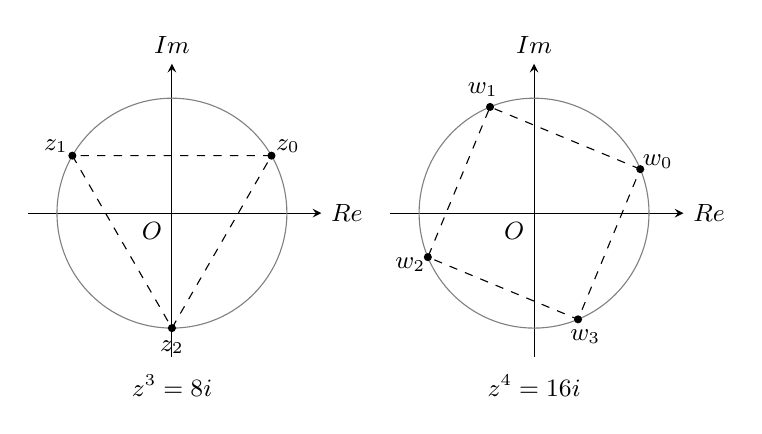
\begin{tikzpicture}[scale=.73,>=stealth,font=\small]
\begin{scope}
\draw[->] (-2.5,0)--(2.6,0) node[right]{\(\operatorname{Re}\)};
\draw[->] (0,-2.5)--(0,2.6) node[above]{\(\operatorname{Im}\)};
\draw[gray] (0,0) circle(2);
\draw[dashed] (30:2)--(150:2)--(270:2)--cycle;
\foreach \a/\k in {30/0,150/1,270/2}
 {\fill (\a:2) circle(2pt); \node at (\a:2.33){\(z_{\k}\)};}
\node[below left] at (0,0){\(O\)};
\node at (0,-3){\(z^3=8i\)};
\end{scope}
\begin{scope}[xshift=6.3cm]
\draw[->] (-2.5,0)--(2.6,0) node[right]{\(\operatorname{Re}\)};
\draw[->] (0,-2.5)--(0,2.6) node[above]{\(\operatorname{Im}\)};
\draw[gray] (0,0) circle(2);
\draw[dashed] (22.5:2)--(112.5:2)--(202.5:2)--(292.5:2)--cycle;
\foreach \a/\k in {22.5/0,112.5/1,202.5/2,292.5/3}
 {\fill (\a:2) circle(2pt); \node at (\a:2.33){\(w_{\k}\)};}
\node[below left] at (0,0){\(O\)};
\node at (0,-3){\(z^4=16i\)};
\end{scope}
\end{tikzpicture}
\end{center}


% ITEM: vector-fifth-roots-cosine
\solutionitem{vector-fifth-roots-cosine}{习题3.9（10）}
设\(\omega = e^{2 \pi i / 5}\)，证明\(1 + \omega + \omega^{2} + \omega^{3} + \omega^{4} = 0\)，并由此求\(\cos \frac{2 \pi}{5}\)的值。
\solutionanswer
由\(\omega^5=1,\omega\ne1\)，有
\[
1+\omega+\omega^2+\omega^3+\omega^4
=\frac{\omega^5-1}{\omega-1}=0.
\]
其中\(\omega^4=\overline\omega,\omega^3=\overline{\omega^2}\)。将共轭项合并，得到
\[
1+2\cos\frac{2\pi}5+2\cos\frac{4\pi}5=0.
\]
设\(c=\cos(2\pi/5)\)，用二倍角公式化为
\[
4c^2+2c-1=0.
\]
由于\(0<2\pi/5<\pi/2\)，取正根，故
\[
\cos\frac{2\pi}5=\frac{\sqrt5-1}4.
\]


% ITEM: vector-complex-loci
\solutionitem{vector-complex-loci}{习题3.9（11）}
说明下列集合表示什么图形，并写出相应的直角坐标方程：\\
\exercisesubitem{1}\(\left| z - \left( 1 + i \right) \right| = 2\)；\\
\exercisesubitem{2}\(\left| z - 1 \right| = \left| z + 1 \right|\)；\\
\exercisesubitem{3}\(\operatorname{Re} \left( \left( 1 - i \right) z \right) = 1\)。
\solutionanswer
设\(z=x+yi\)。

\exercisesubitem{1}表示圆心为\((1,1)\)、半径为\(2\)的圆，方程为
\[
(x-1)^2+(y-1)^2=4.
\]
\exercisesubitem{2}表示点\((1,0),(-1,0)\)的垂直平分线，即虚轴，方程为\(x=0\)。

\exercisesubitem{3}由
\[
(1-i)(x+yi)=(x+y)+(y-x)i,
\]
得直线\(x+y=1\)。


% ITEM: vector-equilateral-vertices
\solutionitem{vector-equilateral-vertices}{习题3.9（12）}
已知不同的两点\(A , B\)对应复数\(a , b\)。求以\(A B\)为边的两个正三角形的第三个顶点，并求它们的重心。
\solutionanswer
将边向量\(b-a\)绕\(A\)旋转\(\pm\pi/3\)，就得到两个第三顶点：
\[
c_\pm=a+e^{\pm\pi i/3}(b-a)
=\frac{a+b}2\pm\frac{\sqrt3}{2}i(b-a).
\]
两个重心分别为
\[
g_\pm=\frac{a+b+c_\pm}3
=\frac{a+b}2\pm\frac{\sqrt3}{6}i(b-a).
\]
两种符号对应边\(AB\)的两侧。式中的\(i(b-a)\)垂直于边，因而也直接给出了第三顶点与重心到边中点的方向和距离。


% ITEM: vector-triangle-area-angle
\solutionitem{vector-triangle-area-angle}{习题3.9（13）}
点\(A , B , C\)分别对应\(1 + i\)，\(4 + i\)，\(2 + 3 i\)。用复数求\(\triangle A B C\)的面积与\(\angle B A C\)的余弦。
\solutionanswer
有\(b-a=3,c-a=1+2i\)，所以
\[
\overline{b-a}(c-a)=3+6i.
\]
虚部给出有向面积的两倍，实部给出数量积，因此
\[
S_{\triangle ABC}=\frac12|6|=3,\qquad
\cos\angle BAC=\frac3{3\sqrt5}=\frac1{\sqrt5}.
\]


% ITEM: vector-circle-distance-extrema
\solutionitem{vector-circle-distance-extrema}{习题3.9（14）}
设\(\left| z - 1 \right| = 2\)，求\(\left| z \right|\)的最大值与最小值，并求取到极值时的\(z\)。
\solutionanswer
点\(z\)在以\(1\)为圆心、半径为\(2\)的圆上。由三角不等式及其反向形式，
\[
1=\bigl||z-1|-1\bigr|\le|z|\le|z-1|+1=3.
\]
在\(z=-1\)时取到最小值\(1\)，在\(z=3\)时取到最大值\(3\)。两点均满足题设圆的方程；由等号对应的共线方向，也知这分别是全部取等点。


% ITEM: vector-real-linear-complex-form
\solutionitem{vector-real-linear-complex-form}{习题3.9（15） *}
将\(\mathbb{C}\)看成二维实线性空间。证明任意线性变换都可以写成\(T \left( z \right) = \alpha z + \beta \overline{z}\)，其中\(\alpha , \beta \in \mathbb{C}\)。若它在基\(1 , i\)下的矩阵为\(\left[ \begin{smallmatrix}p & q \\ r & s\end{smallmatrix} \right]\)，求\(\alpha , \beta\)。
\solutionanswer
一个实线性变换由\(u=T(1),v=T(i)\)决定。对\(z=x+yi\)，有
\[
T(z)=xu+yv,\qquad
x=\frac{z+\overline z}2,\quad y=\frac{z-\overline z}{2i}.
\]
代入并按\(z,\overline z\)合并：
\[
T(z)=\frac{u-iv}2z+\frac{u+iv}2\overline z.
\]
所以取\(\alpha=(u-iv)/2,\beta=(u+iv)/2\)即可。代入\(z=1,i\)也说明这两个系数唯一。

给定矩阵意味着\(u=p+ri,v=q+si\)，故
\[
\boxed{\quad
\alpha=\frac{p+s+i(r-q)}2,\qquad
\beta=\frac{p-s+i(r+q)}2.\quad}
\]
其中\(\beta=0\)时才只需乘以一个固定复数；共轭项使这一表达式能够涵盖一般的实线性变换。
\par
